\section{投机解码系统实现}

\subsection{草稿端实现}

本文的草稿端部署在 Android 设备上，负责在当前已接受前缀基础上提出候选词元。系统在本地推理能力之上抽象出草稿会话接口，Android 端通过 \texttt{start / draft / apply / close} 维护跨轮次草稿状态。

Android 客户端提供本地推理、远程推理和投机解码三类运行入口。在投机解码模式下，客户端需要配置桌面端验证服务地址，并显示当前运行模式、模型组合和诊断日志路径，便于实验过程中确认跨设备协同链路是否处于预期状态。客户端界面如图 \ref{fig:android-app-spec-ui} 所示。

\begin{figure}[H]
  \centering
  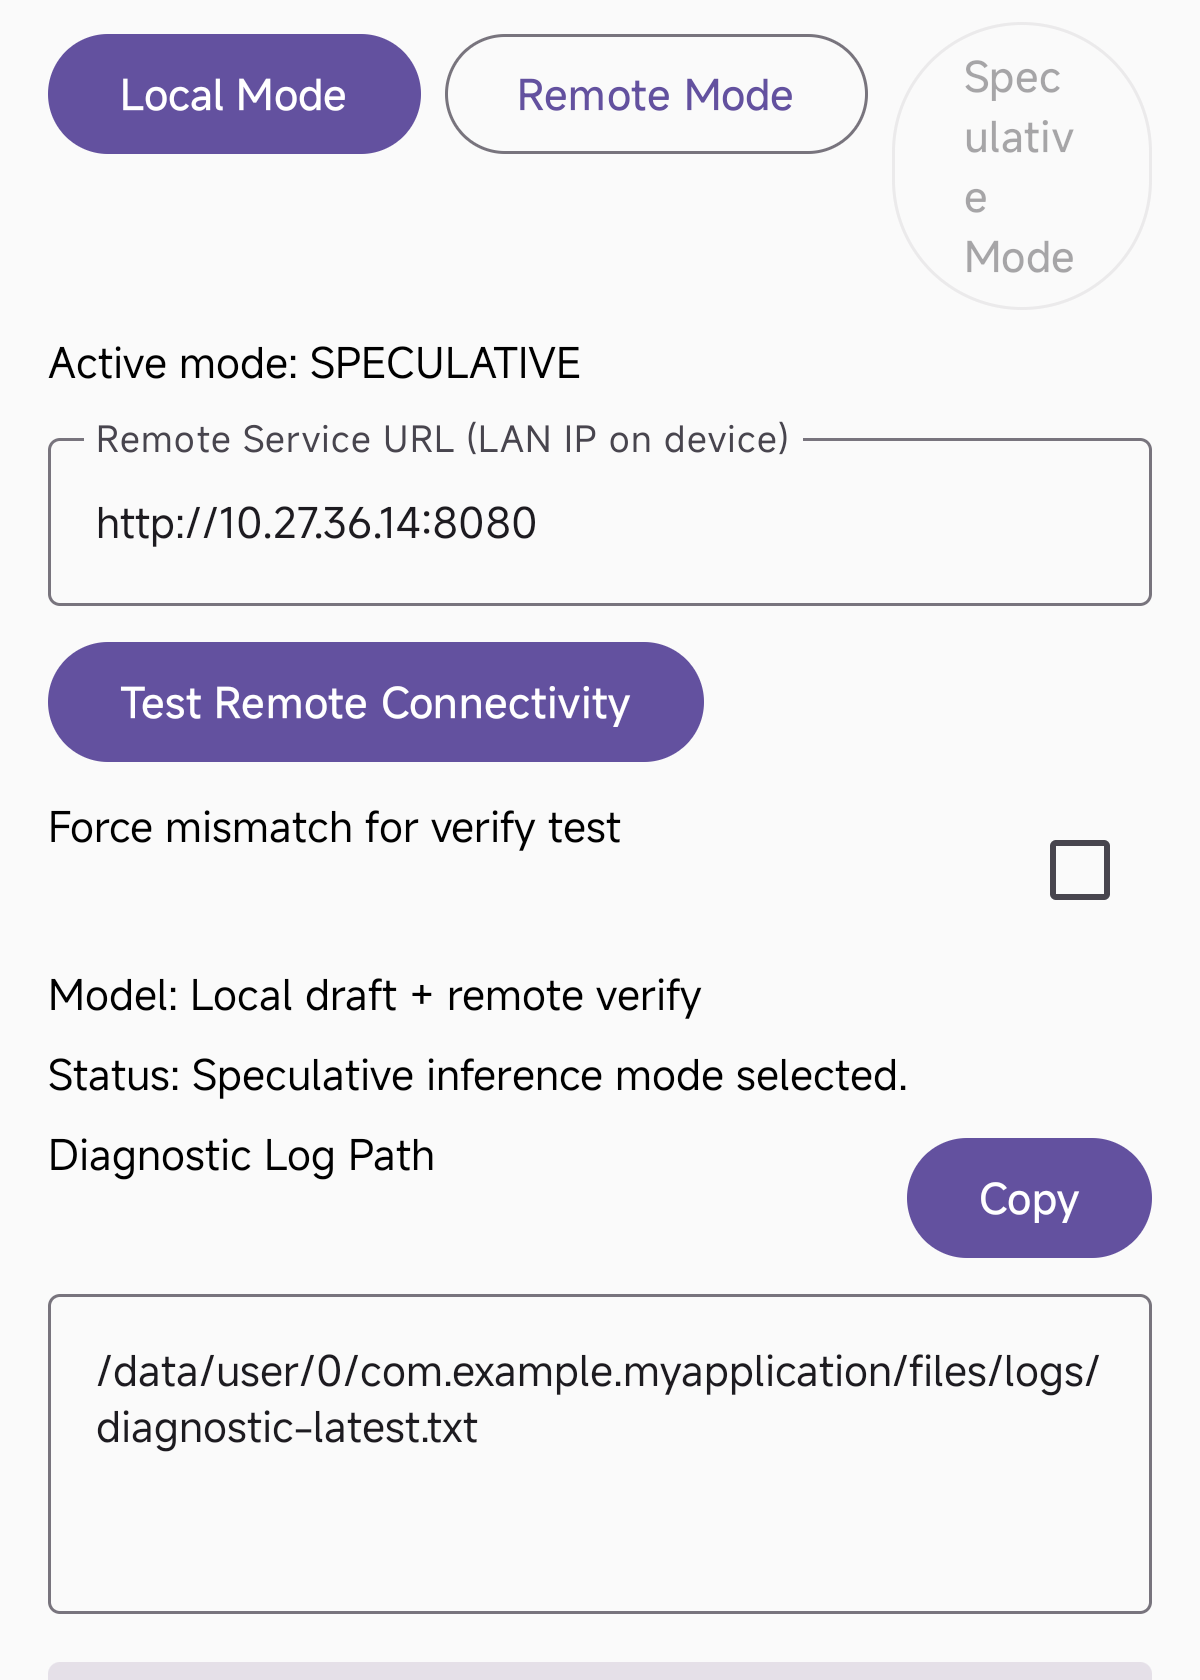
\includegraphics[width=.60\textwidth,height=.45\textheight,keepaspectratio]{figures/android-app-spec-ui-paper-crop.png}
  \caption{Android 客户端投机解码模式界面}
  \label{fig:android-app-spec-ui}
\end{figure}

草稿会话以已接受前缀作为权威状态。每轮提案前，Android 端根据目标侧返回的接受数量和修正词元更新本地会话；每轮提案后，未被目标侧确认的候选词元不写入权威前缀。实现上，草稿端需要完成三项操作：其一，根据已接受词元推进本地上下文；其二，在发生拒绝时回滚未提交尾部；其三，在新的权威前缀上继续生成下一轮候选。该流程用于避免草稿侧沿未确认分支继续生成。

草稿端支持线性提案和分支扩展的草稿树。线性提案用于提交一条候选路径，适合观察基本接受率和单轮推进长度；草稿树用于在若干深度保留多个候选分支。草稿树节点记录词元 id、父子关系、节点概率、累计分支得分和最佳候选索引等信息，目标侧据此在多个候选分支之间执行验证。该结构使候选组织方式与验证逻辑解耦，便于在相同协议下比较线性提案和树形提案。

\subsection{目标端实现}

目标端部署在桌面端推理服务中，负责根据当前已接受前缀对草稿提案进行验证。目标端维护跨轮次验证状态，使同一投机会话中的多次 \texttt{propose} 请求都在连续上下文中执行。

系统在桌面端服务中引入独立的目标会话状态对象。该对象保存已接受文本、目标词元进度、验证模式、运行时后端、调用计数、缓存命中和会话连续性信息。目标验证器每次接收候选后，先读取目标会话中的权威前缀和词元进度，再调用目标模型运行时计算候选位置的目标分布，最后把验证结果写回会话状态。

目标验证器直接围绕草稿端提交的真实词元 id 执行验证。对于线性提案，目标端按候选顺序检查每个词元在当前前缀下是否可接受；对于树形提案，目标端依据候选树结构选择可验证路径，并返回本次验证可提交的词元数量和必要的修正词元。验证结果统一封装为 \texttt{acceptedCount}、\texttt{rejectedIndex} 和 \texttt{correctionTokenId} 等字段，Android 端据此完成提交、回滚和下一轮提案准备。

\subsection{候选生成与验证机制实现}

系统采用线性提案与树形提案并存的候选组织方式。在线性提案中，Android 端一次发送一组候选词元，桌面端按顺序逐个验证：若提案中前若干词元被目标侧接受，则这些词元进入权威前缀；一旦出现拒绝位置，则返回拒绝位置和修正词元。线性提案的实现重点是保持候选顺序、接受计数和回滚位置的一致性。

在树形提案中，草稿端为若干深度保留多个候选分支，目标侧结合树结构执行验证。树形候选在同一轮请求中覆盖多个局部可能性，候选命中概率取决于这些分支与目标分布的重合程度。实现上，树节点需要携带父子关系和候选得分，目标端则根据树结构恢复候选路径，并统计草稿树节点数量、最佳路径节点数和候选重叠情况，用于评估树形提案的覆盖效果。

\texttt{propose} 结果包含接受数量、拒绝位置、修正词元 id 及辅助统计字段。不同候选组织方式共用这组返回语义，上层流程无需感知底层候选结构差异。

\subsection{真实词元对齐与运行时优化实现}

词元空间统一是端云协同投机解码的基本技术条件。Android 草稿侧与桌面端目标侧必须使用一致的真实词元 id 表示候选与修正，否则标准接受机制难以稳定实现\cite{li2024eagle}。

在本文系统中，Android 草稿侧导出真实词元提案和真实词元草稿树，桌面端在验证器边界上直接读取和处理真实词元 id。统一真实词元空间后，系统基于目标概率与草稿概率关系执行接受判定，并在拒绝时引入基于观测残差的修正选择方案。跨设备提案、验证和修正由此使用同一词元表示，避免因文本重编码造成候选偏移。

运行时连续性直接影响系统性能。Android 端通过草稿会话快照、已验证词元提交、未提交尾部回滚和轻量状态恢复降低重复维护成本。桌面端通过目标会话持续化、线程预算设置、会话启动参数对齐和请求字段精简减少每轮验证器的中间开销。上述实现不改变投机解码的接受语义，但决定每轮提案和验证之间需要付出的状态维护成本。
